% !TeX root = RJwrapper.tex
\title{latrend: A Framework for Clustering Longitudinal Data}


\author{by Niek Den Teuling, Steffen Pauws, and Edwin van den Heuvel}

\maketitle

\abstract{%
Clustering of longitudinal data is used to explore common trends among subjects over time. In this paper, we focus on cases where the sole repeated measurement of interest is numeric. Various R packages have been introduced throughout the years for identifying clusters of longitudinal patterns, summarizing the variability in trajectories between subjects in terms of one or more trends. We introduce the R package latrend as a framework for the unified application of methods for longitudinal clustering, enabling comparisons between methods with minimal coding. The package also serves as an interface to commonly used packages for clustering longitudinal data, including dtwclust, flexmix, kml, lcmm, mclust, mixAK, and mixtools. This enables researchers to easily compare different approaches, implementations, and method specifications. Furthermore, researchers can build upon the standard tools provided by the framework to quickly implement new cluster methods, enabling rapid prototyping.
}

\section{Introduction}\label{sec:intro}

In this work, we consider the case where subjects are repeatedly measured on the same variable over a period of time. This type of data is referred to as longitudinal data. In this paper, we focus on the repeated measurement of a single numeric variable, although in other applications, longitudinal measurements may be ordinal or even categorical (e.g., sequence analysis), and comprise multiple variables. No two subjects are identical, and therefore observations made across subjects may develop differently over time. Usually, longitudinal datasets are represented by a single general trend, i.e., an average representative trajectory indicating the expected change and variability over time. However, there may be structural deviations from the trend caused by observed and unobserved factors, or the distribution of random deviations is difficult to model parametrically.

Clustering longitudinal data is a practical approach for exploring or representing the variability between subjects in more detail \citep{hamaker2012researchers}. Here, the variability is summarized in terms of a manageable number of common trends, which are identified in an unsupervised manner from the data using a cluster algorithm. The approach is especially useful for exploring datasets involving a large number of trajectories, where a visual inspection of the trajectories would be impractical. In essence, the data are assumed to comprise several groups, each with a different longitudinal data generating mechanism. It differs from cross-sectional clustering due to the need to account for the dependency between observations within subjects, and the possible temporal correlation in the repeated measurements.

The exploration of subgroups in longitudinal studies is of interest in many domains. Examples include recidivism behavior in criminology, the development of adolescent antisocial behavior or substance use in psychology, and medication adherence in medicine. An example application that we will demonstrate further in this paper is the exploration of the different ways in which patients with sleep apnea adhere to positive airway pressure (PAP) therapy over time. Here, therapy adherence is measured in terms of the number of hours of sleep during which the therapy is used, recorded daily. Patients exhibit different levels of adherence to the therapy, depending on many factors such as their sleep schedule, motivation, self-efficacy, and the perceived importance of therapy \citep{cayanan2019review}. Moreover, patients may exhibit a different level of change over time, depending on their initial usage and their ability to adjust to the therapy. To account for the many possibly unobserved factors involved, researchers have used longitudinal clustering to summarize the between-subject variability in terms of longitudinal patterns of therapy adherence \citep{babbin2015identifying, denteuling2021latent, yi2022identifying}.

A number of packages have been created in R \citep{rcoreteam2021r} that can be used for clustering longitudinal data. However, for researchers analyzing a novel case study, choosing the best method or implementation is not straightforward due to the inherent exploratory nature of such an analysis. Considering that each of these packages has been created to fulfill a gap in the capabilities of other existing implementations or approaches, there is value in comparing the results for new case studies at hand. In any case, the evaluation of different approaches across packages is an activity of considerable effort, as the methods, inputs, estimation procedure, and cluster representations differ greatly between packages.

The aim of the \CRANpkg{latrend} package is to facilitate the exploration of heterogeneity in a longitudinal dataset on a numeric variable of interest, through a variety of cluster methods from various fields of research in a standardized manner. The package provides a unifying framework, enabling users to specify, estimate, select, compare, and evaluate any supported longitudinal cluster method in an easy and consistent way, with minimal coding. Most importantly, users can easily compare results between different approaches, or run a simulation study. A second aim of \CRANpkg{latrend} is to enable users to extend the framework with new methods or add support for other existing methods. The \CRANpkg{latrend} package is available from the Comprehensive R Archive Network (CRAN) at (\url{https://CRAN.R-project.org/package=latrend}) and on GitHub at (\url{https://github.com/niekdt/latrend}).

Currently, a total of 18 methods for longitudinal clustering are supported. To provide support for such a variety of approaches, the \CRANpkg{latrend} package interfaces with an extensive set of packages that provide methods that are applicable for clustering longitudinal data, including \CRANpkg{akmedoids} \citep{Adepeju2020akmedoids}, \CRANpkg{crimCV} \citep{Nielsen2018crimCV}, \CRANpkg{dtwclust} \citep{sardaespinosa2019time}, \CRANpkg{flexmix} \citep{gruen2008flexMix}, \CRANpkg{funFEM} \citep{Bouveyron2015funFEM}, \CRANpkg{kml} \citep{genolini2015kml}, \CRANpkg{lcmm} \citep{proustlima2017estimation}, \CRANpkg{mclust} \citep{Scrucca2016mclust}, \CRANpkg{mixAK} \citep{Komarek2009New}, and \CRANpkg{mixtools} \citep{benaglia2009mixtools}. In this way, we build upon the cluster packages created by the R community. Support has also been added for MixTVEM; a mixture model proposed and implemented as an R script by \citet{dziak2015modeling}.

To the best of our knowledge, such a comprehensive package does not yet exist in the context of clustering longitudinal data. The \CRANpkg{latrend} package has similar aspirations as the \CRANpkg{flexmix} package \citep{gruen2008flexMix}, which also provides an extensible framework for (multilevel) clustering. However, the scope of our package is purposefully broader, to facilitate users to apply approaches from various fields of research. Our framework is agnostic to the specification, estimation, and representation used by the methods.

The paper is organized as follows. A short overview of different approaches to clustering longitudinal data is given in Section \hyperref[sec:methods]{2}. In Section \hyperref[sec:design]{3}, the design principles and high-level structure of the framework are described. The usage of the package is demonstrated in Section \hyperref[sec:demo]{4}. Section \hyperref[sec:extension]{5} describes three ways in which users can implement their own cluster methods. Lastly, a summary and future steps are presented in Section \hyperref[sec:discussion]{6}.

\section{Methods}\label{sec:methods}

We will briefly describe common general approaches to clustering longitudinal data, and the main strengths of these approaches. For brevity, we do not go into the specifics of any of the packages. We refer to the accompanying articles of these packages for further details. Starting with the aspects that all approaches have in common, let the repeated observations of the trajectory from subject \(i\) be denoted by \[\mathbf{y}_i = (y_{i1}, y_{i2}, ..., y_{iJ_i}),\] where \(y_{ij}\) is a numerical value of some variable of interest, \(t_{ij}\) is the measurement time, and \(J_i\) is the number of observations of trajectory \(\mathbf{y}_i\) for subject \(i\).

Regardless of the approach, any method for clustering longitudinal data approximates the dataset heterogeneity in terms of a set of \(K\) clusters, with each cluster representing a proportion \(\pi_k\) of the population, with \(\pi_k > 0\) and \(\sum_{k = 1}^K \pi_k = 1\). The clusters may be discovered by identifying groupings of similar subjects, based on their trajectory. Typically, a cluster method is estimated for a given number of clusters, specified by the user. By applying a cluster method for a different number of clusters, the most appropriate number of clusters can then be determined for the respective data.

Subjects are generally assumed to belong to a single cluster. Therefore, many cluster methods partition the subjects into \(k\) mutually exclusive sets \(I_1, I_2, ..., I_K\), where \(I_k\) denotes the set of subjects to belong to cluster \(k\), with \(\bigcup_{k=1}^{K}I_{k}=I\). Depending on the application, it may be desirable to identify a representation for each cluster, also referred to as the cluster center, which provides a summary of the cluster. This representation may be obtained from the averaged representation of all the subjects assigned to the respective cluster, by designating a representative subject, or through the cluster representation defined by the method, if applicable.

Other cluster methods allow for overlapping clusters, commonly referred to as soft or fuzzy clustering. Here, subjects may belong to multiple clusters, with a certain degree or weight to which subjects belong to each cluster. In the case of model-based clustering \citep{mcnicholas2010model}, the clusters are represented by a mixture of statistical models, for which cluster membership is expressed as a probability. In applications where each subject is assumed to belong to one cluster, subjects are typically assigned to the cluster with the highest subject-specific posterior probability, referred to as modal assignment.

\subsection{Cross-sectional clustering}\label{cross-sectional-clustering}

In a cross-sectional cluster approach, also referred to as a raw-data-based approach \citep{liao2005clustering}, the different observation moments are treated as separate features for a standard cluster algorithm, i.e., as if we are conducting a cross-sectional cluster analysis. In standard cluster algorithms such as \(k\)-means, the features are assumed to be independent, although this is generally not a strict requirement. The temporal independence assumption made in this approach yields a non-parametric representation of the trajectories. This makes it a useful approach for an exploratory analysis without any prior assumptions on the shape of the trajectories. The main limitation of this approach is that observations must be aligned between trajectories, i.e., measured at the same respective moments in time. Consequently, missing observations should be imputed.

An example of a cross-sectional approach is longitudinal \(k\)-means (KmL). KmL applies the \(k\)-means cluster algorithm directly to the observations. The cluster trajectories are determined by the averaged observations of trajectories assigned to the respective cluster. The method is implemented in the \CRANpkg{kml} package by \citet{genolini2015kml}.

A model-based cross-sectional approach is seen in longitudinal latent profile analysis (LLPA), otherwise known as longitudinal latent class analysis \citep{muthen2004latent}. Here, Gaussian mixture modeling is used to describe each moment in time as a normally distributed random variable. A dataset with trajectories each comprising \(J\) observations is thus described by \(J\) random variables, each modeling the response distribution at a different moment in time. Gaussian mixture models can be estimated using, for example, the \CRANpkg{mclust} package by \citet{Scrucca2016mclust}. In the simplest case, the \(J\) observations are modeled as being independent and the variance is shared between clusters, but by relaxing constraints on the covariance matrix, temporal correlations and different cluster shapes can be accounted for.

\subsection{Distance-based clustering}\label{distance-based-clustering}

Distance-based cluster algorithms operate on the pairwise distance between trajectories. These methods take a distance matrix of pairwise trajectory distances as input, where the choice of the distance metric, i.e., the dissimilarity measure, is left to the user. Examples of cluster algorithms that use this approach include \(k\)-medoids and agglomerative hierarchical clustering.

Given the trajectories of subject \(a\) and \(b\), the distance metric is denoted by \(d(\mathbf{y}_a, \mathbf{y}_b)\). As an example, the Euclidean distance \[d(\mathbf{y}_a, \mathbf{y}_b) = \sqrt{\sum_{j} (y_{bj} - y_{aj})^2}.\] may be used as the distance metric. Cross-sectional clustering is a special case of distance-based clustering where a raw-data distance metric is used.

The approach is commonly used for time series clustering\footnote{Clustering longitudinal data can be regarded as a special case of time series clustering where the time series have a common starting point.}, and the list of available distance metrics that have been proposed over the past decades is extensive \citep{aghabozorgi2015time}. A distance function can be specified to account for one or more temporal aspects of interest, e.g., mean level, changes over time, variability, autocorrelation, spectral components, and entropy. Many dissimilarity metrics are implemented in the \CRANpkg{dtwclust} package \citep{sardaespinosa2019time}.

\subsection{Regression-based clustering}\label{regression-based-clustering}

In regression-based clustering, the longitudinal dataset is modeled by a regression model comprising a mixture of submodels \citep{de2008model}. It is also referred to as latent-class trajectory modeling. This approach comprises a versatile class of (semi-)parametric methods. Most importantly, the shape of the trajectories can be represented using a parametric model, requiring fewer parameters compared to a non-parametric approach. Measurements can be taken at different times between subjects, and covariates can be accounted for. Moreover, users can incorporate assumptions into the modeling of the trajectories and clusters, such as the distribution of the response variable, the within-cluster variability, and heteroskedasticity.

A straightforward example of regression-based clustering involves modeling the population as a mixture of cluster trajectory models. This is referred to as group-based trajectory modeling (GBTM) or latent-class growth analysis (LCGA). It is essentially a mixture of linear regression models, with \begin{equation} \label{eqn:gbtm_y}
  y_{ij} = \mathbf{x}_{ij} \mathbf{\beta}_k + \varepsilon_{ijk} \quad \textrm{for } i \in I_k,
\end{equation} where \(\mathbf{x}_{ij}\) is the \(N \times B\) design matrix of \(B\) covariates, \(\mathbf{\beta}_k\) are the \(B\) group-specific coefficients, and \(\varepsilon_{ijk}\) is the normally distributed residual error with zero mean and constant variance \(\sigma_k^2\) which may be specified to differ between clusters. The design matrix contains covariates of time, enabling the model to describe the change in response over time. External covariates can be included to further explain the dependent variable. The expected values of a trajectory, assuming the trajectory belongs to cluster \(k\), is given by \begin{equation}
  \label{eqn:gbtm}
  E(y_{ij} | C_i = k) = \mathbf{x}_{ij} \mathbf{\beta}_k.
\end{equation} GBTM is available, for example, in the packages \CRANpkg{lcmm} \citep{proustlima2017estimation} and \CRANpkg{crimCV} \citep{Nielsen2018crimCV}.

A popular form of regression-based clustering that does consider within-cluster variability is growth mixture modeling (GMM) \citep{muthen2004latent}, which represents a mixture of multilevel models. Here, the within-cluster variability is modeled by allowing for subject-specific deviations from the cluster center, e.g., a deviation in the intercept. Using a linear mixed modeling approach, the trajectories for cluster \(k\) are given by \begin{equation}
  y_{ij} = \mathbf{x}_{ij} \mathbf{\beta}_k + \mathbf{z}_{ij} \mathbf{u}_{ki} + \varepsilon_{ijk} \quad \textrm{for } i \in I_k.
\end{equation} Here, \(\mathbf{z}_{ij}\) is the \(N \times U\) design matrix for the \(U\) random effects, and \(\mathbf{u}_{ki}\) are the subject-specific random coefficients for cluster \(k\). The random effects are assumed to be normally distributed with mean zero and variance-covariance matrix \(\Sigma_k\). The expected values of a trajectory, assuming the trajectory belongs to cluster \(k\), is given by \begin{equation}
  \label{eqn:gmm}
  E(y_{ij} | C_i = k, \mathbf{u}_{i}) = \mathbf{x}_{ij} \mathbf{\beta}_k + \mathbf{z}_{ij} \mathbf{u}_{ki}.
\end{equation} GMM is available in packages such as \CRANpkg{lcmm} \citep{proustlima2017estimation}, \CRANpkg{mixtools} \citep{benaglia2009mixtools}, and \CRANpkg{mixAK} \citep{Komarek2009New}.

\subsection{Feature-based clustering}\label{feature-based-clustering}

In a feature-based approach, each trajectory is independently represented by a set of temporal characteristics (i.e., features, coefficients), for example, the mean, variability, and change over time \citep{liao2005clustering}. The trajectories are then clustered based on the features or coefficients using a cross-sectional cluster algorithm. This can be regarded as a special case of distance-based clustering, but with a domain-tailored distance function. This approach has the advantage of allowing users to easily combine arbitrary features of interest. The approach is used, for example, by the anchored \(k\)-medoids algorithm provided by the \CRANpkg{akmedoids} package \citep{Adepeju2020akmedoids}. Here, the trajectories are represented using linear regression models, and are clustered based on the model coefficients.

Compared to the rather time-intensive regression-based clustering approach, the trajectory models only need to be estimated once. A disadvantage compared to regression-based clustering is that the reliability of the trajectory coefficients depends on the available data per trajectory. This approach therefore generally requires a greater number of observations per subject to yield similar results.

\subsection{Identifying the number of clusters}\label{identifying-the-number-of-clusters}

Due to the exploratory nature of clustering, the number of clusters is typically not known in advance. Moreover, most of the cluster methods require the user to specify the number of clusters. The preferred number of clusters for the respective method can be determined by estimating the method for an increasing number of clusters, followed by comparing the solutions by means of an evaluation metric. In such a comparison for a particular method, the interpretation of the metric is consistent across the solutions, as they all originate from the same method specification.

Many metrics are available, although they may not be defined for each type of method. For example, in distance-based methods, the solutions are typically evaluated in terms of the separation between clusters. Cluster separation is measured by the distance between trajectories or cluster trajectories, e.g., using the average Silhouette width (ASW) \citep{rousseeuw1987silhouettes} or the Dunn index \citep{arbelaitz2013extensive}. In contrast, a regression-based approach typically has no notion of the distance between trajectories, but instead measures the likelihood of the overall regression model on the given data, enabling the use of likelihood-based evaluation such as the Bayesian information criterion (BIC), Akaike information criterion (AIC), or likelihood ratio test \citep{vandernest2020overview}. Specific to cluster regression methods where the longitudinal observations are modeled at the subject level, assessing the solution in terms of the residual errors of the trajectories may be of interest. Examples of such metrics include the mean absolute error (MAE) and root mean squared error (RMSE). For probabilistic assignments these metrics may be weighted by the posterior probability of the trajectories, denoted as WMAE and WRMSE, respectively.

Overall, the preferred metric depends on the type of method under consideration and the case study domain. In the case of evaluation between different types of methods, a metric should be selected which is defined for both types of method, which may rule out many of the options. Users are advised to follow recommendations from literature for the respective method. Moreover, it is advisable to use the evaluation metric merely as guidance in identifying the preferred solution, as a trade-off between the number of clusters and the interpretability of the solution. Lastly, it is worthwhile to factor in domain knowledge into the selection of cluster solutions \citep{nagin2018group}.

\subsection{Comparing methods}\label{methods-compare}

The approaches may yield considerably different results, arising from fundamental differences in the temporal representation and similarity criterion of the methods. Moreover, some approaches are more applicable to certain measurement moments, sample sizes, trajectory shapes and cluster sizes than others. To guide users towards an initial choice for a suitable approach, we have listed some of the general strengths and limitations of the different approaches in Table \ref{tbl:compare}. Note that even for methods of the same type of approach, results may differ depending on how the trajectories are represented, trajectory similarity is measured, or how clusters are formed. Considering that the most suitable approach or method is typically not known in advance, it is advisable to evaluate and compare the solutions between methods to identify the most suitable method for the respective case study. The resulting solutions can then be compared using an external evaluation metric.

A useful starting point in comparing the preferred solutions between methods is to evaluate the similarity between the cluster partitions. After all, if both candidate methods find a similar cluster partition, this would indicate that both methods find the same grouping despite representational differences. In contrast, if the cluster partitions are dissimilar, it may suggest that either a hybrid approach could be of interest, or that one method is preferred over the other.

The similarity between cluster partitions of two methods can be assessed using partition similarity metrics such as the adjusted Rand index (ARI) \citep{hubert1985comparing}, variance of information, or the split-join index. These metrics are applicable to any method and are even applicable when the solutions have a mismatching number of clusters. In some case studies, a ground truth may be available in the form of a reference cluster partition. Partition similarity metrics such as the ARI may then be used to identify the solution that most closely resembles the ground truth. Alternatively, one may obtain a partial ground truth by manually annotating a subset of the trajectories based on domain knowledge.

Solutions may be compared further by assessing the compactness of the clusters or the separation between clusters on a common distance metric, for example using the average Silhouette width or the Dunn index. This is useful to identify the method that is best at identifying distinct subgroups.

\renewcommand{\arraystretch}{2}

\begin{longtable}[]{@{}
  >{\raggedright\arraybackslash}p{(\linewidth - 4\tabcolsep) * \real{0.0823}}
  >{\raggedright\arraybackslash}p{(\linewidth - 4\tabcolsep) * \real{0.5152}}
  >{\raggedright\arraybackslash}p{(\linewidth - 4\tabcolsep) * \real{0.3983}}@{}}
\caption{Summary of the general strengths and limitations of the different approaches to longitudinal clustering. \label{tbl:compare}}\tabularnewline
\toprule\noalign{}
\begin{minipage}[b]{\linewidth}\raggedright
Approach
\end{minipage} & \begin{minipage}[b]{\linewidth}\raggedright
Strengths
\end{minipage} & \begin{minipage}[b]{\linewidth}\raggedright
Limitations
\end{minipage} \\
\midrule\noalign{}
\endfirsthead
\toprule\noalign{}
\begin{minipage}[b]{\linewidth}\raggedright
Approach
\end{minipage} & \begin{minipage}[b]{\linewidth}\raggedright
Strengths
\end{minipage} & \begin{minipage}[b]{\linewidth}\raggedright
Limitations
\end{minipage} \\
\midrule\noalign{}
\endhead
\bottomrule\noalign{}
\endlastfoot
Cross-sectional & \begin{minipage}[t]{\linewidth}\raggedright
\begin{itemize}
\tightlist
\item
  Suitable for initial exploration due to no assumptions on the shape of the cluster trajectories
\item
  Low sample size requirement
\item
  Very fast to estimate
\end{itemize}
\end{minipage} & \begin{minipage}[t]{\linewidth}\raggedright
\begin{itemize}
\tightlist
\item
  Requires time-aligned trajectories of equal length
\item
  Requires complete data
\item
  Does not account for the temporal relation of observations
\end{itemize}
\end{minipage} \\
Distance-based & \begin{minipage}[t]{\linewidth}\raggedright
\begin{itemize}
\tightlist
\item
  Flexible in the choice of distance metric(s)
\item
  Trajectory distance matrix only needs to be computed once
\item
  Fast to estimate
\end{itemize}
\end{minipage} & \begin{minipage}[t]{\linewidth}\raggedright
\begin{itemize}
\tightlist
\item
  Distance matrix computation is not practical for a large number of trajectories
\item
  Pairwise comparison of trajectories is more sensitive to noise
\item
  Many distance metrics require time-aligned trajectories
\end{itemize}
\end{minipage} \\
Regression-based & \begin{minipage}[t]{\linewidth}\raggedright
\begin{itemize}
\tightlist
\item
  Low sample size requirements due to inclusion of parametric assumptions \citep{martin2015growth}
\item
  Can handle missing data
\item
  Can handle trajectories of unequal length and variable time
\item
  Can account for covariates
\item
  Relatively robust to trajectories that do not fit the representation
\end{itemize}
\end{minipage} & \begin{minipage}[t]{\linewidth}\raggedright
\begin{itemize}
\tightlist
\item
  May be challenging to estimate (convergence problems) \citep{denteuling2021comparison}
\item
  Computationally intensive to estimate
\end{itemize}
\end{minipage} \\
Feature-based & \begin{minipage}[t]{\linewidth}\raggedright
\begin{itemize}
\tightlist
\item
  Temporal features only needs to be computed once
\item
  Very fast to estimate
\item
  Fast alternative to regression-based approach given a sufficiently large sample size \citep{denteuling2021comparison}
\end{itemize}
\end{minipage} & \begin{minipage}[t]{\linewidth}\raggedright
\begin{itemize}
\tightlist
\item
  Sensitive to trajectories that do not fit the representation
\item
  Trajectory-independent feature estimation is more sensitive to observational outliers
\end{itemize}
\end{minipage} \\
\end{longtable}

\section{Software design}\label{sec:design}

We begin by providing a high-level description of the framework, outlining the main functionality of the classes. A step-by-step demonstration of the framework is given in the next section. The software is built on an object-oriented paradigm using the S4 system, available in the \pkg{methods} package \citep{rcoreteam2021r}. The framework is designed to provide a standardized way of specifying, estimating, and evaluating different longitudinal cluster methods. This is achieved by defining two interfaces: the \texttt{lcMethod} interface is used for defining the specification and estimation logic of a method. The \texttt{lcModel} interface represents the result of an estimated method. Using these two interfaces, we can then define method-agnostic estimation procedures for applying a specified method to a given dataset, yielding a method result. This estimation procedure is implemented by the \texttt{latrend()} function. For example, users can specify a growth mixture model (GMM) through a \texttt{lcMethodLcmmGMM} object, specifying the GMM and the estimation settings. The resulting estimated GMM is represented by a \texttt{lcModelLcmmGMM} object.

A key advantage of having stand-alone estimation procedures is that it ensures all methods take the same data format as input, and allows for more procedures to be implemented which automatically support all implemented methods. There are additional procedures implemented in the package, including repeated estimation via \texttt{latrendRep()}, batch estimation via \texttt{latrendBatch()}, and standard non-parametric bootstrap sampling via \texttt{latrendBoot()}.

\subsection{Dataset input}\label{dataset-input}

We have selected the \texttt{data.frame} in long format as the preferred representation for longitudinal datasets. Here, each row represents an observation for a trajectory at a given time, possibly for multiple covariates. The trajectory and time of an observation are indicated in separate columns. This format can represent irregularly timed measurements, a variable number of observations per trajectory, and an arbitrary number of covariates of different types. Since not all datasets are readily available in this format, the \texttt{latrend()} estimation procedures handle data input by calling the generic \texttt{transformLatrendData()} function. Currently, this transformation is only defined for \texttt{matrix} input. Users can implement the method to add support for other longitudinal data types.

\subsection{\texorpdfstring{The \texttt{lcMethod} class}{The lcMethod class}}\label{subsec:lcmethod}

The \texttt{lcMethod} class has two purposes. The first purpose is to record the method specification, defined by the method parameters and other settings, referred to as the method arguments. The second purpose is to provide the logic for estimating the method for the specified arguments and given data. \texttt{lcMethod} objects are immutable. Users only interact with a \texttt{lcMethod} object for retrieving method arguments, or for creating a new specification with modified arguments. This functionality is provided by the base \texttt{lcMethod} class.

The base class also stores the method arguments in a list, inside the \texttt{arguments} slot. The method arguments can be of any type. The names of subclasses are prefixed by ``\emph{lcMethod}''. Subclasses can validate the model arguments against the data by overriding the \texttt{validate()} function. Due to the specific internal structure of a \texttt{lcMethod} object, constructors are defined for creating \texttt{lcMethod} objects of a specific class for a given set of arguments. In \texttt{lcMethod} implementations that are a wrapper around an existing cluster package function, the method arguments are simply passed to the package function. The required arguments and their default values are obtained from the formal function arguments of the package function at runtime.

The evaluation of the method arguments is delayed until the method estimation process. This enables a \texttt{lcMethod} object to be printed in an easily readable way, where the original argument expressions or calls are shown, instead of the evaluation result. This is useful when an argument takes on a function or complex data structure, and it reduces the memory footprint when a large set of method permutations is generated and serialized, such as in a simulation study.

The method estimation process is implemented through six generic functions: \texttt{prepareData()}, \texttt{compose()}, \texttt{validate()}, \texttt{preFit()}, \texttt{fit()}, and \texttt{postFit()}. The purpose of each step is explained in Section \hyperref[sec:extension]{5}. There are several advantages to this design. Firstly, the structure enables the method estimation process to be checked at each step. Secondly, splitting the estimation logic into processing steps encourages shorter functions with clearer functionality, resulting in more readable code. Thirdly, the steps enable optimizations in the case of repeated method estimation, for which the \texttt{prepareData()} function only needs to be called once. Lastly, in case of an update to the \texttt{lcModel} post-processing step, the \texttt{postFit()} function can be applied to previously obtained \texttt{lcModel} objects.

\subsubsection{Supported methods}\label{supported-methods}

An overview of the currently available methods that can be specified is given in Table \ref{tbl:methods}. The \texttt{lcMethodGCKM} class implements a feature-based approach, based on representing the trajectories through a linear mixed model specified in the \CRANpkg{lme4} package \citep{Bates2015Fitting}.

\renewcommand{\arraystretch}{1.5}

\begin{longtable}[]{@{}
  >{\raggedright\arraybackslash}p{(\linewidth - 4\tabcolsep) * \real{0.1594}}
  >{\raggedright\arraybackslash}p{(\linewidth - 4\tabcolsep) * \real{0.5000}}
  >{\raggedright\arraybackslash}p{(\linewidth - 4\tabcolsep) * \real{0.3333}}@{}}
\caption{The list of currently supported methods for clustering longitudinal data, in alphabetical order. The methods in the bottom row represent generic approaches which can be adapted. Class names are prefixed by ``lcMethod''. \label{tbl:methods}}\tabularnewline
\toprule\noalign{}
\begin{minipage}[b]{\linewidth}\raggedright
Class (\texttt{lcMethod})
\end{minipage} & \begin{minipage}[b]{\linewidth}\raggedright
Method
\end{minipage} & \begin{minipage}[b]{\linewidth}\raggedright
Package
\end{minipage} \\
\midrule\noalign{}
\endfirsthead
\toprule\noalign{}
\begin{minipage}[b]{\linewidth}\raggedright
Class (\texttt{lcMethod})
\end{minipage} & \begin{minipage}[b]{\linewidth}\raggedright
Method
\end{minipage} & \begin{minipage}[b]{\linewidth}\raggedright
Package
\end{minipage} \\
\midrule\noalign{}
\endhead
\bottomrule\noalign{}
\endlastfoot
\texttt{Akmedoids} & Anchored \emph{k}-medoids & \CRANpkg{akmedoids} \citep{Adepeju2020akmedoids} \\
\texttt{CrimCV} & Group-based trajectory modeling of count data & \CRANpkg{crimCV} \citep{Nielsen2018crimCV} \\
\texttt{Dtwclust} & Dynamic time warping & \CRANpkg{dtwclust} \citep{sardaespinosa2019time} \\
\texttt{Flexmix} & Interface to FlexMix framework & \CRANpkg{flexmix} \citep{gruen2008flexMix} \\
\texttt{FlexmixGBTM} & Group-based trajectory modeling & \CRANpkg{flexmix} \citep{gruen2008flexMix} \\
\texttt{FunFEM} & funFEM & \CRANpkg{funFEM} \citep{Bouveyron2015funFEM} \\
\texttt{GCKM} & Feature-based clustering using growth curve modeling and \emph{k}-means & \CRANpkg{lme4} \citep{Bates2015Fitting} \\
\texttt{KML} & longitudinal \emph{k}-means & \CRANpkg{kml} \citep{genolini2015kml} \\
\texttt{LcmmGBTM} & Group-based trajectory modeling & \CRANpkg{lcmm} \citep{proustlima2017estimation} \\
\texttt{LcmmGMM} & Growth mixture modeling & \CRANpkg{lcmm} \citep{proustlima2017estimation} \\
\texttt{LMKM} & Feature-based clustering using linear regression and \emph{k}-means & \\
\texttt{MclustLLPA} & Longitudinal latent profile analysis & \CRANpkg{mclust} \citep{Scrucca2016mclust} \\
\texttt{MixAK\_GLMM} & Mixture of generalized linear mixed models & \CRANpkg{mixAK} \citep{Komarek2009New} \\
\texttt{MixtoolsGMM} & Growth mixture modeling & \CRANpkg{mixtools} \citep{benaglia2009mixtools} \\
\texttt{MixtoolsNPRM} & Non-parametric repeated measures clustering & \CRANpkg{mixtools} \citep{benaglia2009mixtools} \\
\texttt{MixTVEM} & Mixture of time-varying effects models & \\
\texttt{Random} & Random partitioning & \\
\texttt{Stratify} & Stratification rule & \\
\texttt{Feature} & Feature-based clustering & \\
\end{longtable}

Additionally, a partitioning of trajectories can be specified without an estimation step through the \texttt{lcModelPartition} and \texttt{lcModelWeightedPartition} classes, providing trajectories with a cluster membership or membership weight, respectively.

\subsection{\texorpdfstring{The \texttt{lcModel} class}{The lcModel class}}\label{subsec:lcmodel}

The \texttt{lcModel} class represents the estimated cluster solution. It is designed to function as any other model fitted in R. Here, the word ``model'' should be taken in the broadest sense of the word, where any resulting cluster partitioning represents the data, and thereby is regarded as a model of said data. Users can apply the familiar functions from the \pkg{stats} package \citep{rcoreteam2021r} where applicable, including the \texttt{predict()}, \texttt{plot()}, \texttt{summary()}, \texttt{fitted()}, and \texttt{residuals()} functions. Furthermore, \texttt{lcModel} objects support functions for obtaining the cluster representation, such as the cluster proportions, sizes, names, and trajectories.

The base \texttt{lcModel} class facilitates basic functionality such as providing a solution summary and providing functionality for computing predictions or fitted values. The two most important functions that characterize the class are the \texttt{predict()} and \texttt{postprob()} functions. These functions are used to derive the cluster trajectories, the posterior probabilities of the trajectories, and cluster proportions.

The base class stores information regarding the model, including the estimated \texttt{lcMethod} object, the \texttt{call} that was used to estimate the method, the date and time when the method was estimated, the total estimation time, and a text label for differentiating solutions. Users should not update the slots of the base class directly, except for the \texttt{tag} slot, which is intended as a convenient way of assigning custom meta data to the \texttt{lcModel}.

The names of subclasses are prefixed by ``\emph{lcModel}''. Subclasses generally have little need for adding new slots, as most of the functionality resides inside the class functions, such that results and statistics are computed dynamically. This enables fitted \texttt{lcModel} objects to be modified retroactively, e.g., for correcting implementation errors that are discovered at a later stage.

In the \texttt{lcModel} subclass implementations that are based on an underlying R package, the subclass serves as a wrapper around the underlying package model. The underlying model is exposed via the \texttt{getModel()} function so that users can still benefit from the specialized functionality provided by the underlying package.

\subsection{The metric interfaces}\label{subsec:metric}

There is a vast number of metrics available in literature. To provide access to as many metrics as possible, and to enable users to add missing metrics as needed, we define an interface for the computation of metrics. Users can replace or extend the metrics with custom implementations. To ensure a consistent output across all metrics, the output of metric functions must be scalar. Note that some metrics may be undefined for certain types of methods, in which case \texttt{NA} is returned (e.g., likelihood-based metrics such as the AIC and BIC are only defined for model-based methods). Currently, the framework supports any of the applicable metrics from the packages \CRANpkg{clusterCrit} \citep{Desgraupes2018clusterCrit} and \CRANpkg{mclustcomp} \citep{You2018mclustcomp}. The list of supported internal and external metrics is obtained via the \texttt{getInternalMetricNames()} and \texttt{getExternalMetricNames()} functions, respectively. Metrics can be added or updated via the \texttt{defineInternalMetric()} and \texttt{defineExternalMetric()} functions.

\section{Using the package}\label{sec:demo}

We illustrate the main capabilities of the package through a step-by-step exploratory cluster analysis on the longitudinal dataset named \texttt{PAP.adh} which is included with the package. This synthetic dataset was simulated based on the real-world study reported by \citet{yi2022identifying}, who investigated the longitudinal CPAP therapy usage patterns of patients with obstructive sleep apnea since the start of their treatment. They identified three distinct patterns of therapy adherence: patients who were adherent to the therapy and stable in their usage (``Adherent''), patients who were consistently non-adherent (``Non-adherent''), and patients who improved their usage over time (``Improvers''). We used the growth mixture model fit reported by the authors to simulate new patients, yielding the \texttt{PAP.adh} dataset.

The goal of the analysis is to identify the common patterns of adherence and to establish the most suitable method for the data out of those considered. For brevity, the description of the package function arguments used in the demonstration below is limited to the main arguments. We refer users to the package documentation to learn more about other optional arguments.

The \texttt{PAP.adh} dataset comprises records of the weekly average hours of therapy usage of 301 patients in their first 13 weeks of therapy. Therapy usage ranges between 0 and 9.5 hours, with a mean of 4.5 hours. The \texttt{PAP.adh} dataset is represented by a \texttt{data.frame} in long format, with each row representing the observation of a patient at a specific week (1 to 13).

\begin{verbatim}
library("latrend")
data("PAP.adh")
head(PAP.adh, n = 3)
\end{verbatim}

\begin{verbatim}
#>   Patient Week UsageHours    Group
#> 1       1    1   6.298703 Adherers
#> 2       1    2   5.916080 Adherers
#> 3       1    3   5.022241 Adherers
\end{verbatim}

The \texttt{Patient} column indicates the trajectory to which the observation belongs. The \texttt{UsageHours} column represents the averaged hours of usage in the respective therapy week, denoted by the \texttt{Week} column. The true cluster membership per trajectory is indicated by the \texttt{Group} column.

Throughout the analysis, there are several occasions during which the trajectory identifier and time columns would need to be specified. Instead of passing the column names to each function, we can set the default index columns using the \texttt{options} mechanism. Keep in mind that this is only recommended during interactive use.

\begin{verbatim}
options(latrend.id = "Patient", latrend.time = "Week")
\end{verbatim}

We can visualize the patient trajectories using the \texttt{plotTrajectories()} function, shown in Figure \ref{fig:data}. As the ground truth is known in our synthetic example, we specified the cluster membership of the trajectories via the \texttt{cluster} argument, resulting in a stratified visualization.

\begin{verbatim}
plotTrajectories(PAP.adh, response = "UsageHours", cluster = "Group")
\end{verbatim}

\begin{figure}

{\centering 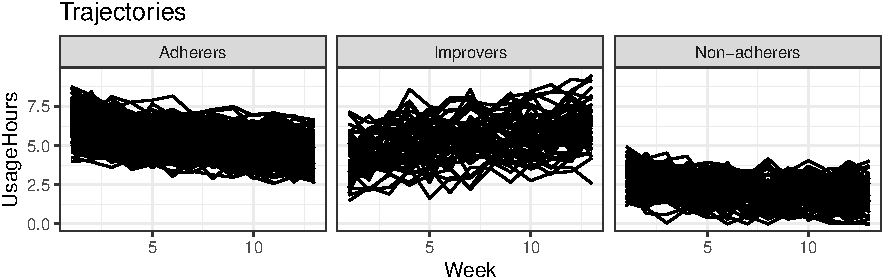
\includegraphics{figures/data-1} 

}

\caption{The trajectories from the `PAP.adh` dataset, by reference group.}\label{fig:data}
\end{figure}

\subsection{Specifying methods}\label{specifying-methods}

We first specify the methods to be evaluated. The first method of interest in this case study is KmL, selected for its flexibility in identifying patterns of any shape. The KmL method is available in the framework through the \texttt{lcMethodKML} class, which serves as a wrapper around the \texttt{kml()} function of the \CRANpkg{kml} package \citep{genolini2015kml}. The KmL method is specified through the \texttt{lcMethodKML()} constructor function.

\begin{verbatim}
kmlMethod <- lcMethodKML(response = "UsageHours", nClusters = 2)
kmlMethod
\end{verbatim}

\begin{verbatim}
#> lcMethodKML specifying "longitudinal k-means (KML)"
#>  time:           getOption("latrend.time")
#>  id:             getOption("latrend.id")
#>  nClusters:      2
#>  nbRedrawing:    20
#>  maxIt:          200
#>  imputationMethod:"copyMean"
#>  distanceName:   "euclidean"
#>  power:          2
#>  distance:       function() {}
#>  centerMethod:   meanNA
#>  startingCond:   "nearlyAll"
#>  nbCriterion:    1000
#>  scale:          TRUE
#>  response:       "UsageHours"
\end{verbatim}

Note that any unspecified arguments have been set to the default values defined by the \CRANpkg{kml} package. The method arguments can be accessed using the \texttt{\$} or \texttt{{[}{[}} operator. Requested arguments are evaluated unless disabled by the argument \texttt{eval\ =\ FALSE}. As can be seen in the method output below, the time index column is obtained from the \texttt{options} mechanism by default.

\begin{verbatim}
kmlMethod$time
\end{verbatim}

\begin{verbatim}
#> [1] "Week"
\end{verbatim}

\begin{verbatim}
kmlMethod[["time", eval = FALSE]]
\end{verbatim}

\begin{verbatim}
#> getOption("latrend.time")
\end{verbatim}

Next, we specify the other methods of interest. We use a variety of approaches that are applicable to this type of data. We evaluate a feature-based approach based on LMKM as implemented in \texttt{lcMethodLMKM}, a distance-based dynamic time warping approach via \texttt{lcMethodDtwclust} based on the \CRANpkg{dtwclust} package, and the regression-based approaches via the \texttt{lcMethodLcmmGBTM} and \texttt{lcMethodLcmmGMM} methods based on the \CRANpkg{lcmm} package \citep{proustlima2017estimation}. We specify the distance-based approach using dynamic time warping. For LMKM, GBTM and GMM, we model the trajectories using an intercept and slope\footnote{For methods supporting formula input, the response variable is automatically determined from the response of the formula.}. Moreover, GBTM and GMM are specified to use a shared diagonal variance-covariance matrix. The GMM defines a random patient intercept.

\begin{verbatim}
dtwMethod <- lcMethodDtwclust(response = "UsageHours", distance = "dtw_basic")
lmkmMethod <- lcMethodLMKM(formula = UsageHours ~ Week)
gbtmMethod <- lcMethodLcmmGBTM(fixed = UsageHours ~ Week,
  mixture = ~ Week, idiag = TRUE)
gmmMethod <- lcMethodLcmmGMM(fixed = UsageHours ~ Week,
  mixture = ~ Week, random = ~ 1, idiag = TRUE)
\end{verbatim}

The method arguments of a \texttt{lcMethod} object cannot be modified. Instead, a new specification is created from the existing one with the updated method arguments. Any \texttt{lcMethod} object can be used as a prototype for creating a new specification with new, modified, or removed arguments using the \texttt{update()} function. As an example, if we would like to respecify KmL to identify three clusters, this can be done by updating the existing specification as follows:

\begin{verbatim}
kml3Method <- update(kmlMethod, nClusters = 3)
\end{verbatim}

As the number of clusters is generally not known in advance, we need to fit the methods for a range of number of clusters. Generating specifications for a series of argument values can be done via the \texttt{lcMethods()} function, which outputs a \texttt{list} of updated \texttt{lcMethod} objects from a given prototype. We specify each method for up to six clusters\footnote{Only one to four clusters were estimated for GBTM and GMM due to the relatively excessive computation time} using:

\begin{verbatim}
kmlMethods  <- lcMethods(kmlMethod,  nClusters = 1:6)
lmkmMethods <- lcMethods(lmkmMethod, nClusters = 1:6)
dtwMethods  <- lcMethods(dtwMethod,  nClusters = 2:6)
gbtmMethods <- lcMethods(gbtmMethod, nClusters = 1:4)
gmmMethods  <- lcMethods(gmmMethod,  nClusters = 1:4)
length(gmmMethods)
\end{verbatim}

\begin{verbatim}
#> [1] 4
\end{verbatim}

\subsection{Fitting methods}\label{fitting-methods}

Using the previously created method specifications, we can estimate the methods for the \texttt{PAP.adh} data. For estimating a single method, we can use the \texttt{latrend()} function. The function optionally accepts an \texttt{environment} through the \texttt{envir} argument for evaluating the method arguments within a specific environment. The output of the function is the fitted \texttt{lcModel} object.

\begin{verbatim}
lmkm2 <- latrend(lmkmMethod, data = PAP.adh)
summary(lmkm2)
\end{verbatim}

\begin{verbatim}
#> Longitudinal cluster model using lmkm
#> lcMethodLMKM specifying "lm-kmeans"
#>  time:           "Week"
#>  id:             "Patient"
#>  nClusters:      2
#>  center:         function (x) {    mean(x, na.rm = TRUE)}
#>  standardize:    `scale`
#>  method:         "qr"
#>  model:          TRUE
#>  y:              FALSE
#>  qr:             TRUE
#>  singular.ok:    TRUE
#>  contrasts:      NULL
#>  iter.max:       10
#>  nstart:         1
#>  algorithm:      `c("Hartigan-Wong", "Lloyd", "Forgy", "M
#>  formula:        UsageHours ~ Week
#> 
#> Cluster sizes (K=2):
#>           A           B 
#> 166 (55.1%) 135 (44.9%) 
#> 
#> Number of obs: 3913, strata (Patient): 301
#> 
#> Scaled residuals:
#>     Min.  1st Qu.   Median     Mean  3rd Qu.     Max. 
#> -2.52815 -0.67127 -0.06772  0.00000  0.54587  4.04438
\end{verbatim}

Instead of needing to update a method prior to calling \texttt{latrend()}, the arguments to be updated can also be passed directly to \texttt{latrend()}. Here, we estimate the LMKM method for three clusters.

\begin{verbatim}
lmkm3 <- latrend(lmkmMethod, nClusters = 3, data = PAP.adh)
\end{verbatim}

Alternatively, we can achieve the same result by updating the previously estimated two-cluster solution.

\begin{verbatim}
lmkm3 <- update(lmkm2, nClusters = 3)
\end{verbatim}

\subsubsection{Batch estimation}\label{batch-estimation}

The \texttt{latrendBatch()} function estimates a list of method specifications. This is useful for evaluating a method for a range of number of clusters, as we have defined above using the \texttt{lcMethods()} function. Another use case is the improvement of model convergence and the estimation time by tuning the control parameters. Optimizing such parameters may yield considerably improved convergence or considerably reduced estimation time on larger datasets. Many of the methods have settings for the number of random starts, maximum number of iterations, and convergence criteria. However, because such control settings are specific to each method, we will not cover this.

The inputs to the \texttt{latrendBatch()} function are a list of \texttt{lcMethod} objects, and a list of datasets. The output is an \texttt{lcModels} object, representing a list of the fitted \texttt{lcModel} objects for each dataset. A seed is specified to ensure reproducibility of the examples.

\begin{verbatim}
lmkmList <- latrendBatch(lmkmMethods, data = PAP.adh, seed = 1)
lmkmList
\end{verbatim}

\begin{verbatim}
#> List of 6 lcModels with
#>   .name .method       seed nClusters
#> 1     1    lmkm  762473831         1
#> 2     2    lmkm 1762587819         2
#> 3     3    lmkm 1463113723         3
#> 4     4    lmkm 1531473323         4
#> 5     5    lmkm 1922000657         5
#> 6     6    lmkm 1985277999         6
\end{verbatim}

When printing a \texttt{lcModels} object, the content is shown as a table of method specifications. By default, only arguments which differ between the models are shown. The table can also be obtained as a \texttt{data.frame} by calling \texttt{as.data.frame()}. We now fit the other methods in the same manner.

\begin{verbatim}
dtwList <- latrendBatch(dtwMethods, data = PAP.adh, seed = 1)
\end{verbatim}

For the repeated estimation of more computationally intensive methods, we can speed up the process by using parallel computation. By setting \texttt{parallel\ =\ TRUE}, the \texttt{latrendBatch()} function will use the parallel back-end of the \CRANpkg{foreach} package \citep{weston2022foreach}. To make use of this functionality, we first need to configure the parallel back-end:

\begin{verbatim}
nCores <- parallel::detectCores(logical = FALSE)
if (.Platform$OS.type == "windows") {
  doParallel::registerDoParallel(parallel::makeCluster(nCores))
} else {
  doMC::registerDoMC(nCores)
}
\end{verbatim}

The methods can then be estimated in parallel using:

\begin{verbatim}
kmlList  <- latrendBatch(kmlMethods,
  data = PAP.adh, parallel = TRUE, seed = 1)
gbtmList <- latrendBatch(gbtmMethods,
  data = PAP.adh, parallel = TRUE, seed = 1)
gmmList  <- latrendBatch(gmmMethods,
  data = PAP.adh, parallel = TRUE, seed = 1)
\end{verbatim}

\subsection{Evaluation}\label{evaluation}

\subsubsection{Assessing a cluster result}\label{assessing-a-cluster-result}

A cluster result is useful only when it describes the data adequately. There are various aspects on which the cluster result can be evaluated, depending on the method and analysis domain:

\begin{itemize}
\tightlist
\item
  The identified solution may not be reliable when the method estimation procedure did not converge. Convergence can be checked via the \texttt{converged()} function.
\item
  The cluster solution may comprise empty clusters or clusters with a negligible proportion of trajectories. In such a case, re-estimating the method may yield a better solution. Alternatively, one should consider fitting the method with a lower number of clusters.
\item
  The cluster trajectories may be assessed visually to determine whether the identified patterns are sufficiently distinct.
\item
  The prediction error may help to determine to what degree trajectories are represented by one of the clusters.
\end{itemize}

As shown in the previous section, the summary of an \texttt{lcModel} object shows the method arguments values, cluster sizes, cluster proportions, cluster names, and the standardized residuals. By default, the residuals are computed from the difference between the reference values and the predictions outputted by \texttt{fitted()}, conditional on the most likely trajectory assignments. For methods that do not provide trajectory-specific predictions, the fitted values are determined from the cluster trajectories.

The cluster trajectories can be obtained using the \texttt{clusterTrajectories()} function, returning a \texttt{data.frame}. The cluster trajectories can be plotted via \texttt{plot()} or \texttt{plotClusterTrajectories()}. The three-cluster LMKM solution is visualized in Figure \ref{fig:trends}. For parametric cluster methods, a more concise representation of the model can be obtained from the model coefficients, using \texttt{coef()}.

\begin{verbatim}
plot(lmkm3, linewidth = 1)
\end{verbatim}

\begin{figure}

{\centering 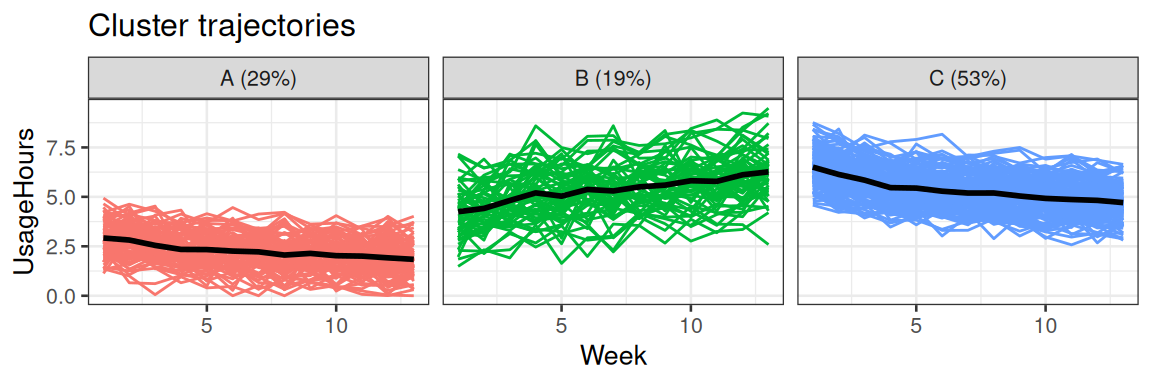
\includegraphics{figures/trends-1} 

}

\caption{The cluster trajectories of the three-cluster solution identified by LMKM, created by running plot(lmkm3).}\label{fig:trends}
\end{figure}

Assigning descriptive names to the clusters can help to increase the readability of the cluster result, which is especially useful for solutions with many clusters. The \texttt{clusterNames()} function can be used to retrieve or change the cluster names.

\begin{verbatim}
clusterNames(lmkm3) <- c("Struggling", "Increasing", "Decreasing")
\end{verbatim}

The most likely cluster for each of the trajectories is obtained using the \texttt{trajectoryAssignments()} function, which outputs a \texttt{factor} with the cluster names as its levels. For soft-cluster representations, the cluster assignments are determined by the cluster with the highest probability, based on the posterior probability matrix. An alternative approach can be specified through the \texttt{strategy} argument. For example, the \texttt{which.weight()} function assigns a random cluster weighted by the proportions. The \texttt{which.is.max()} function from the \CRANpkg{nnet} package \citep{venables2002modern} returns the most likely cluster, breaking ties at random.

The posterior probability matrix can be obtained from the \texttt{postprob()} function\footnote{For methods that only support modal assignment, the posterior probability matrix only comprises 0 and 1.}. For probabilistic methods, it can be used to gauge the cluster separation, i.e., the certainty of assignment. The posterior probability is also important in the post-hoc analysis for accounting for the uncertainty in cluster assignment.

When it comes to longitudinal representation, the minimum functionality that is available for all \texttt{lcModel} objects is the prediction of the cluster trajectories at the given moments in time. The prediction has been implemented for underlying packages that lack this functionality. For non-parametric methods such as KmL or LLPA, linear interpolation is used when time points are requested which are not represented by the cluster centers.The available functionality differs between methods.

All \texttt{lcModel} objects support the standard model functions from the standard \pkg{stats} package, including \texttt{fitted()}, \texttt{residuals()}, and \texttt{predict()}. These functions are primarily of interest for methods that have a notion of a group or individual trajectory prediction error, such as for the regression-based approaches like GBTM and GMM. The \texttt{fitted()} function returns the expected values for the response variable for the data on which the model was estimated. By default, only the values for the most likely cluster are given. However, for \texttt{clusters\ =\ NULL}, a matrix of predictions is outputted, where each column represents the predictions of the respective cluster.

The \texttt{predict()} function computes trajectory- and cluster-specific predictions for the given input data.

\begin{verbatim}
predict(lmkm3, newdata = data.frame(Week = c(1, 10), Cluster = "Decreasing"))
\end{verbatim}

\begin{verbatim}
#>        Fit
#> 1 2.919423
#> 2 2.024865
\end{verbatim}

The \texttt{predictPostprob()} and \texttt{predictAssignments()} functions compute the posterior probability and cluster membership for new trajectories, respectively. As this is not a common use case for cluster methods, most of the underlying packages do not provide this functionality. For demonstration purposes, we have implemented the functionality for the \texttt{lcModelKML} class.

Using the metric interface defined in Section \hyperref[sec:methods]{2}, we can compute a variety of internal metrics through the \texttt{metric()} function:

\begin{verbatim}
metric(lmkm3, c("MAE", "RMSE", "Dunn", "ASW"))
\end{verbatim}

\begin{verbatim}
#>        MAE       RMSE       Dunn        ASW 
#> 0.74262252 0.94094913 0.09173111 0.35605235
\end{verbatim}

\subsubsection{Identifying the number of clusters}\label{identifying-the-number-of-clusters-1}

Using one or more internal metrics of interest, we can assess how the data representation of a method improves or worsens for an increasing number of clusters. In this case study, we will use the Dunn index as the primary metric for the choice of the number of clusters.

The change in metrics for an increasing number of clusters can be visualized via the \texttt{plotMetric()} function, and can help to determine the preferred solution. For brevity, we will only provide a detailed view for the KmL method. We plot the Dunn index, WMAE, and estimation time (in seconds) for the six KmL solutions as follows:

\begin{verbatim}
plotMetric(kmlList, c("Dunn", "WMAE", "estimationTime"))
\end{verbatim}

\begin{figure}

{\centering 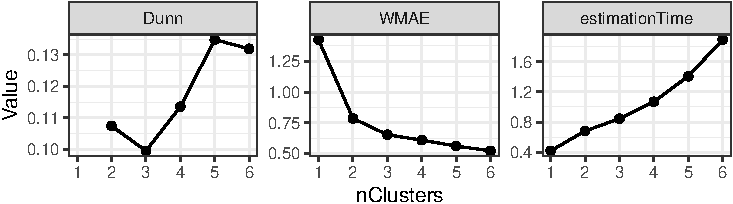
\includegraphics{figures/numclusmetrics-1} 

}

\caption{The Dunn index (higher is better), and WMAE (lower is better) metrics for each of the KmL solutions from 1 to 6 clusters}\label{fig:numclusmetrics}
\end{figure}

The resulting plot is shown in Figure \ref{fig:numclusmetrics}. The Dunn index and WMAE show a rather convincing improvement for an increasing number of clusters\footnote{The Dunn index is not defined for a one-cluster solution.}.

Moreover, we observe that the estimation time increases with the number of clusters. This can be a practical consideration when deciding on the preferred method to use. For much larger datasets, it may be useful to conduct a preliminary analysis on a subset of the data for possibly ruling out methods which are too computationally intensive in relation to the results.

We can obtain the metric values for each of the models by calling the \texttt{metric()} function.

\begin{verbatim}
metric(kmlList, c("Dunn", "WMAE", "estimationTime"))
\end{verbatim}

\begin{verbatim}
#>         Dunn      WMAE estimationTime
#> 1         NA 1.4261264          0.416
#> 2 0.10737225 0.7850566          0.680
#> 3 0.09944419 0.6523208          0.844
#> 4 0.11353357 0.6081128          1.070
#> 5 0.13487175 0.5598639          1.409
#> 6 0.13196444 0.5209264          1.896
\end{verbatim}

As the preferred solution corresponds to the highest Dunn index, we can obtain the respective model by calling the \texttt{max()} function on the \texttt{lcModels} list object.

\begin{verbatim}
kmlBest <- max(kmlList, "Dunn")
\end{verbatim}

Alternatively, we can select the preferred model using the \texttt{subset()} function. By specifying the \texttt{drop\ =\ TRUE}, the \texttt{lcModel} object is returned instead of a \texttt{lcModels} object.

\begin{verbatim}
kmlBest <- subset(kmlList, nClusters == 5, drop = TRUE)
\end{verbatim}

The identification of the number of clusters is a form of model selection. The same approach can therefore be used for identifying the best cluster representation, e.g., evaluating different formulas for a parametric model, or selecting a different method initialization strategy.

\subsubsection{Comparing methods}\label{comparing-methods}

The optimal number of clusters according to the internal metric can be different for other methods or specifications thereof. Depending on the cluster representation, some methods may require fewer or more clusters to represent the heterogeneity to the same degree. By concatenating the lists of fitted methods, we can create a metric plot that is grouped by the type of method as follows:

\begin{verbatim}
allList <- lcModels(lmkmList, kmlList, dtwList, gbtmList, gmmList)
plotMetric(allList, name = c("Dunn", "WMAE", "BIC", "estimationTime"), group = '.method')
\end{verbatim}

\begin{figure}

{\centering 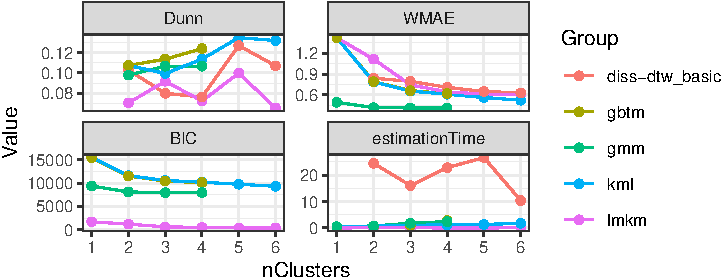
\includegraphics{figures/numclus-1} 

}

\caption{The Dunn index (higher is better), WMAE (lower is better) and BIC (relatively lower is better) for each of the methods and number of clusters}\label{fig:numclus}
\end{figure}

The WMAE and BIC between GBTM and KmL are almost exactly the same, possibly indicating that the methods find a similar solution. If the solutions are found to be practically identical, then one could actually prefer KmL due to its considerably favorable computational scaling with the number of clusters.

We explore the best solution of each method further to better understand how the cluster representations differ between the methods. We can select the preferred \texttt{lcModel} object corresponding to the selected number of clusters for each of the methods using the \texttt{subset()} function.

\begin{verbatim}
kmlBest  <- subset(kmlList,  nClusters == 5, drop = TRUE)
dtwBest  <- subset(dtwList,  nClusters == 5, drop = TRUE)
gbtmBest <- subset(lmkmList, nClusters == 4, drop = TRUE)
lmkmBest <- subset(lmkmList, nClusters == 3, drop = TRUE)
gmmBest  <- subset(gmmList,  nClusters == 3, drop = TRUE)
\end{verbatim}

We can then assess the pairwise ARI between each method using the \texttt{externalMetric()} function. Calling this function on a \texttt{lcModels} list returns a \texttt{dist} object representing a distance matrix. We therefore create a list of the best \texttt{lcModel} for each method, by which we can then determine the pairwise ARI as follows:

\begin{verbatim}
bestList <- lcModels(KmL = kmlBest, DTW = dtwBest,
  LMKM = lmkmBest, GBTM = gbtmBest, GMM = gmmBest)
externalMetric(bestList, name = "adjustedRand") |> signif(2)
\end{verbatim}

\begin{verbatim}
#>       KmL  DTW LMKM GBTM
#> DTW  0.41               
#> LMKM 0.50 0.40          
#> GBTM 0.66 0.31 0.67     
#> GMM  0.49 0.40 0.99 0.68
\end{verbatim}

With all pairwise ARI being at least 0.31, all methods demonstrate some degree of similarity between each other. In particular, the very high ARI of approximately 0.99 between GMM and LMKM implies that the methods grouped the trajectories in a highly similar way.

Secondly, we evaluate the similarity of the cluster trajectories between the methods using the weighted minimum mean absolute error (WMMAE) \citep{denteuling2021comparison}. This metric computes the mean absolute error between each cluster trajectory and its nearest cluster trajectory of the other method, weighted by the size of the respective cluster.

\begin{verbatim}
externalMetric(bestList, name = "WMMAE") |> signif(2)
\end{verbatim}

\begin{verbatim}
#>        KmL   DTW  LMKM  GBTM
#> DTW  0.096                  
#> LMKM 0.130 0.130            
#> GBTM 0.063 0.130 0.091      
#> GMM  0.130 0.130 0.036 0.099
\end{verbatim}

The mean absolute error of 0.091 between the cluster trajectories of GBTM and LMKM is negligible compared to the residual error estimated by GBTM (\(\textrm{SD} = 0.8\)), which indicates that both methods have identified practically the same cluster trajectories. The same applies to GMM and LMKM.

\subsection{Cluster validation}\label{cluster-validation}

Assessing the stability and reproducibility of a cluster method can help to determine whether the identified cluster solution generalizes beyond the data that was used to estimate the method. This is especially relevant for more complex cluster methods involving many parameters, which may not generalize well to new data. This primarily pertains to the number of clusters the method is estimated for, as the number of parameters increases linearly with the number of clusters. Even relatively simple methods can overfit the data when the representation comprises too many clusters in relation to the sample size.

\subsubsection{Cluster stability using repeated estimation}\label{cluster-stability-using-repeated-estimation}

Many of the cluster methods can yield a slightly different solution during each run, depending on the starting conditions. In such cases, by doing a repeated estimation, we can gauge the stability, i.e., consistency, of the method. Comparing repeated estimation results is also useful for selecting the best solution for a given method.

Repeated estimation can be done via the \texttt{latrendRep()} function, where the number of repetitions is specified via the \texttt{.rep} argument. Similar to \texttt{latrend()}, the method arguments can be updated within the function. The function returns a \texttt{lcModels} object, comprising a \texttt{list} of \texttt{lcModel} objects. Here, we only use five repeated estimations to limit the computation time. In practice, a higher number such as 10 or 25 is advisable, depending on the magnitude of instability.

\begin{verbatim}
kmlRepList <- latrendRep(kmlMethod, data = PAP.adh,
  nClusters = 5, .rep = 5, .parallel = TRUE)
summary(metric(kmlRepList, c("Dunn", "WMAE")))
\end{verbatim}

\begin{verbatim}
#>       Dunn             WMAE       
#>  Min.   :0.1286   Min.   :0.5617  
#>  1st Qu.:0.1286   1st Qu.:0.5619  
#>  Median :0.1286   Median :0.5658  
#>  Mean   :0.1311   Mean   :0.5643  
#>  3rd Qu.:0.1349   3rd Qu.:0.5658  
#>  Max.   :0.1349   Max.   :0.5665
\end{verbatim}

The result suggests that the solutions found by KmL are highly consistent on this dataset, in the sense that both metrics demonstrate a negligible level of variability between repeated estimations.

\subsubsection{Cluster stability using bootstrap sampling}\label{cluster-stability-using-bootstrap-sampling}

Instead of assessing the cluster stability across repeated estimation on the same dataset, we can obtain a more generalizable estimate of the cluster stability in a nonparametric way by measuring the cluster stability across different datasets. This form of bootstrap sampling, also referred to as bootstrapping, involves the repeated estimation on simulated datasets generated from the original dataset. It is primarily used for assessing the stability of a method, as measured by one or more internal metrics. Here, complete trajectories are selected at random with replacement from the dataset to generate a new dataset of equal size. Each simulated dataset, referred to as a bootstrap sample in this context, will yield a slightly different solution. This variability between samples can provide an indication of the stability of the cluster method on the overall dataset \citep{hennig2007clusterwise}. Since the repeated estimation is done on new datasets that only partially overlap\footnote{In addition to the challenge of the cluster representations being in a different order between runs, also referred to as label switching.}, this restricts the available external metrics to only those that can compare between different datasets, e.g., the WMMAE.

The \texttt{latrendBoot()} function applies bootstrapping to the given method specification. The \texttt{samples} argument determines the number of times the data is resampled, and a model is estimated. Setting the \texttt{seed} argument ensures that the same sequence of bootstrap samples is generated when redoing the bootstrapping procedure. The output is a \texttt{lcModels} list containing the model for each sample. The estimated methods each have a different \texttt{call} for the \texttt{data} argument such that the original bootstrap training sample can be recreated as needed. This avoids the need for models to store the training data. As an example, we compute 10 bootstrap samples\footnote{In practice, a much greater number of bootstrap samples is recommended (at least 100).} (i.e., repeated fits) in parallel as follows:

\begin{verbatim}
kmlMethodBest <- update(kmlMethod, nClusters = 5)
kmlBootModels <- latrendBoot(kmlMethodBest, data = PAP.adh,
  samples = 10, seed = 1, parallel = TRUE)
head(kmlBootModels, n = 3)
\end{verbatim}

\begin{verbatim}
#> List of 3 lcModels with
#>   .name .method                                        data       seed
#> 1     1     kml  bootSample(PAP.adh, "Patient", 762473831L) 1062140483
#> 2     2     kml bootSample(PAP.adh, "Patient", 1762587819L)  185557490
#> 3     3     kml bootSample(PAP.adh, "Patient", 1463113723L)  934902099
\end{verbatim}

We can now assess the stability of the solutions across the models in terms of metrics of interest. Here, we assess the mean convergence rate, and the quantiles of the WMAE and Dunn metrics.

\begin{verbatim}
bootMetrics <- metric(kmlBootModels, c("converged", "Dunn", "WMAE"))
mean(bootMetrics$converged)
\end{verbatim}

\begin{verbatim}
#> [1] 1
\end{verbatim}

\begin{verbatim}
summary(bootMetrics$Dunn)
\end{verbatim}

\begin{verbatim}
#>    Min. 1st Qu.  Median    Mean 3rd Qu.    Max. 
#>  0.1193  0.1469  0.1512  0.1530  0.1645  0.1852
\end{verbatim}

\begin{verbatim}
summary(bootMetrics$WMAE)
\end{verbatim}

\begin{verbatim}
#>    Min. 1st Qu.  Median    Mean 3rd Qu.    Max. 
#>  0.5326  0.5489  0.5542  0.5530  0.5576  0.5728
\end{verbatim}

As can be seen from the output, there is quite some variability between the estimated solutions across bootstrap samples. This suggests that we should consider estimation with repeated random starts to identify a better and more stable solution.

Lastly, we can compute a similarity matrix for an external metric of interest, containing the pairwise similarity for each model pair.

\begin{verbatim}
wmmaeDist <- externalMetric(kmlBootModels[1:10], name = "WMMAE")
summary(wmmaeDist)
\end{verbatim}

\begin{verbatim}
#>    Min. 1st Qu.  Median    Mean 3rd Qu.    Max. 
#> 0.01594 0.05696 0.07259 0.06952 0.08264 0.11011
\end{verbatim}

Showing that there is only a small degree of discrepancy in the cluster trajectories between bootstrap samples.

\subsubsection{Comparison to ground truth}\label{comparison-to-ground-truth}

We now consider the case where a method is evaluated in a simulation study. In such a study, the ground truth is known, and we can directly evaluate whether the trajectories are clustered correctly. A useful and intuitive measure is the split-join distance \citep{dongen2000performance}, which is an edit distance that measures the number of trajectory reassignments that are needed to go from one partitioning to another. In case of a ground truth, we are only interested in the edit distance from the reference partitioning\footnote{In the one-way edit distance, a solution that has more clusters than the reference can still obtain an edit distance of zero if the extra clusters are a subset of the cluster of the reference.}.

We can obtain the vector of trajectory cluster membership of the \texttt{PAP.adh} from the \texttt{Group} column by selecting the first cluster name of each trajectory, since the cluster membership is stable over time. We then create a \texttt{lcModelPartition} from the computed membership vector. By default, the \texttt{lcModelPartition} generates the cluster representations from the means of the trajectories assigned to the respective cluster.

\begin{verbatim}
refAssignments <- aggregate(Group ~ Patient, data = PAP.adh, FUN = head, n = 1L)
refAssignments$Cluster = refAssignments$Group

refModel <- lcModelPartition(data = PAP.adh,
  trajectoryAssignments = refAssignments, response = "UsageHours")
refModel
\end{verbatim}

\begin{verbatim}
#> Longitudinal cluster model using part
#> lcMethod specifying "undefined"
#> no arguments
#> 
#> Cluster sizes (K=3):
#>     Adherers    Improvers Non-adherers 
#>  162 (53.8%)   56 (18.6%)   83 (27.6%) 
#> 
#> Number of obs: 3913, strata (Patient): 301
#> 
#> Scaled residuals:
#>      Min.   1st Qu.    Median      Mean   3rd Qu.      Max. 
#> -3.894748 -0.643671 -0.009533  0.000000  0.634893  3.590377
\end{verbatim}

We can now compare our selected method solutions to the reference solution using the one-way split-join distance to the reference:

\begin{verbatim}
externalMetric(bestList, refModel, name = "splitJoin.ref", drop = FALSE)
\end{verbatim}

\begin{verbatim}
#>      splitJoin.ref
#> KmL             23
#> DTW             61
#> LMKM             3
#> GBTM             1
#> GMM              2
\end{verbatim}

This shows that, for the \texttt{PAP.adh} dataset, LMKM, GBTM, and GMM achieve a nearly perfect recovery of the cluster memberships, but that GBTM needs more clusters to represent the dataset.

\section{Implementing new methods}\label{sec:extension}

One of the main strengths of the framework is the standard way in which methods are specified, estimated, and evaluated. These aspects make it easy to compare newly implemented methods with existing ones. Using the base classes \texttt{lcMethod} and \texttt{lcModel}, new methods can be implemented with a relatively minimal amount of code, enabling rapid prototyping. These classes provide basic functionality, from which the user can extend certain functions as needed by creating a subclass.

\subsection{Stratification}\label{stratification}

The simplest form of clustering is the stratification of the dataset based on a known factor. This can be the response variable, or any other measure available for each trajectory. This is useful for case studies where there is prior knowledge or expert guidance on how the trajectories should be grouped; either by another factor (e.g., age or gender), or a characteristic of the trajectory (e.g., the intercept, slope, average, or variance).

A stratification approach can be specified using the \texttt{lcMethodStratify()} function, which takes an R expression as input. The expression is evaluated within the \texttt{data.frame} at the trajectory level during the method estimation, so any column present in the data can be used. The expression should resolve to a number or category, indicating the stratum for the respective trajectory.

As an example, we stratify the trajectories by thresholding on the mean hours of usage. This expression returns a \texttt{logical} value which determines the cluster assignment. For categorizing trajectories into more than two clusters, the \texttt{cut()} function can be used. The cluster trajectories are computed by aggregating the trajectories of each cluster at the respective time points. By default, the average is computed, but an alternative center function can be specified via the \texttt{center} argument.

\begin{verbatim}
stratMethod <- lcMethodStratify(response = "UsageHours", stratify = mean(UsageHours) > 4)
stratModel <- latrend(stratMethod, data = PAP.adh)
clusterProportions(stratModel)
\end{verbatim}

\begin{verbatim}
#>         A         B 
#> 0.3156146 0.6843854
\end{verbatim}

\subsection{Feature-based clustering}\label{feature-based-clustering-1}

Feature-based clustering is a flexible and fast approach to clustering longitudinal data, with an essentially limitless choice of trajectory representations. The framework includes a generic feature-based clustering class named \texttt{lcMethodFeature} for quickly implementing this approach.

A \texttt{lcMethodFeature} specification requires two functions: A representation function outputting the trajectory representation \texttt{matrix}, and a cluster function that applies a cluster algorithm to the matrix, returning an \texttt{lcModel} object.

To illustrate the method, we represent each trajectory using a linear model, and we cluster the model coefficients using \(k\)-means. In the representation step, \texttt{lm()} is applied to each trajectory, and the model coefficients are combined into a \texttt{matrix} with the trajectory-specific coefficients on each row. We parameterize the \texttt{lcMethod} implementation by obtaining the model formula from \texttt{method\$formula}. During the method specification, the user therefore needs to define the \texttt{formula} argument. The representation function is as follows:

\begin{verbatim}
repStep <- function(method, data, verbose) {
  repTraj <- function(trajData) {
    lm.rep <- lm(method$formula, data = trajData)
    coef(lm.rep)
  }
  dt <- as.data.table(data)
  coefData <- dt[, as.list(repTraj(.SD)), keyby = c(method$id)]
  coefMat <- as.matrix(subset(coefData, select = -1))
  rownames(coefMat) <- coefData[[method$id]]
  coefMat
}
\end{verbatim}

We implement the cluster step to return a \texttt{lcModelPartition} object based on the cluster assignments outputted by \texttt{kmeans()}. We have parameterized the function by obtaining the number of clusters for \(k\)-means from the \texttt{nClusters} model argument. The cluster function is as follows:

\begin{verbatim}
clusStep <- function(method, data, repMat, envir, verbose) {
  km <- kmeans(repMat, centers = method$nClusters)
  lcModelPartition(response = responseVariable(method), method = method,
    data = data, trajectoryAssignments = km$cluster, center = mean)
}
\end{verbatim}

We can now specify and estimate the feature-based method, including the additionally required arguments. Comparing the estimated model to the preferred KmL model, we see that the solutions have a relatively high degree of overlap.

\begin{verbatim}
tsMethod <- lcMethodFeature(response = "UsageHours", formula = UsageHours ~ Week,
  representationStep = repStep, clusterStep = clusStep)
tsModel <- latrend(tsMethod, data = PAP.adh, nClusters = 5)
externalMetric(tsModel, kmlBest, "adjustedRand")
\end{verbatim}

\begin{verbatim}
#> adjustedRand 
#>    0.6283228
\end{verbatim}

\begin{verbatim}
externalMetric(tsModel, kmlBest, "WMMAE")
\end{verbatim}

\begin{verbatim}
#>      WMMAE 
#> 0.06505086
\end{verbatim}

\subsection{Implementing a method}\label{sec:custommethod}

The framework is designed to support the implementation of new methods, so that users can extend or implement new methods to address their use case. In this section, we describe the high-level steps that are involved in adding support for a method to the framework. Considering the number of lines of code for even a relatively simple cluster method, we do not cover a complete example here. Instead, we only outline the typical set of functions that need to be implemented, together with any relevant input and output assumptions of these functions. For complete examples, see the \texttt{lcMethod}-interface implementations based on external packages, e.g., \texttt{lcMethodKML} or \texttt{lcMethodLcmmGMM}. A step-by-step example of implementing a statistical method in the framework can be found in the vignette included with the package, which can be viewed by running \texttt{vignette("implement",\ package\ =\ \ "latrend")}.

The estimation process of a method is divided into six steps, involving the processing of the method arguments, preparing and validating the data, and fitting the specified method. All steps except for \texttt{fit()} are optional.

\begin{enumerate}
\def\labelenumi{\arabic{enumi}.}
\tightlist
\item
  The \texttt{prepareData()} function transforms the training data into the required format for the internal method estimation code. By default, data is provided in long format in a \texttt{data.frame}. For most implementations, no transformation is therefore needed. Cluster methods for repeated-measures data typically require data to be transformed to \texttt{matrix} format, however.
\item
  The \texttt{compose()} function evaluates the method arguments and returns an updated \texttt{lcMethod} object with the evaluated method arguments. The function can also be used for modifying or even replacing the original \texttt{lcMethod} object for the remainder of the estimation process. This is useful when a method is a special case of a more general method and intends to conceal derivative or redundant arguments from the base class.
\item
  The \texttt{validate()} function enables evaluated method arguments to be checked against the input data. This can be used, for example, for checking whether the data contains the covariates specified in the method formula, or whether an argument has a valid value. For implementations which wrap an underlying package function, this validation is usually not needed as the underlying package already performs validation of the input.
\item
  The \texttt{preFit()} function is intended for processing any arguments prior to fitting. In order for these results to be persistent, they should be returned in an \texttt{environment} object, which will be passed as an input to the \texttt{fit()} function.
\item
  The \texttt{fit()} function is where the internal method is estimated for the given specification to obtain the cluster result. This function is also responsible for creating the corresponding \texttt{lcModel} object. The running time of this function is used to determine the method estimation time.
\item
  The \texttt{postFit()} function takes the outputted \texttt{lcModel} from \texttt{fit()} as input, enabling post-processing to be done. This is used, for example, for computing derivative statistics, or for reducing the memory footprint by stripping redundant data fields from the internal model representation. Preferably, this function is implemented such that it can be called repeatedly, allowing for updates to fitted methods without requiring re-estimation.
\end{enumerate}

The implementation of a method requires defining a new \texttt{lcMethod} class. Usually, a new \texttt{lcModel} class needs to be implemented to handle the result and representation of the fitted method. If the new method only outputs a partitioning, then the \texttt{lcModelPartition} class may be used instead.

\section{Summary and outlook}\label{sec:discussion}

The \CRANpkg{latrend} package facilitates the standardized yet flexible exploration of heterogeneity in longitudinal datasets, with a minimal amount of coding effort. The framework provides functionality for specifying, estimating, and assessing models for clustering longitudinal data. The package builds upon the efforts of the R community by providing an interface to the many methods for clustering longitudinal data across packages. Perhaps most importantly, the \CRANpkg{latrend} package makes it easy to compare between any two cluster methods, enabling users to identify the most suitable method to their use case. To ensure transparent and reproducible research, all decisions and settings that are relevant to the analysis should be reported. A useful checklist for reporting on latent-class trajectory studies is provided by \citet{van2017grolts}, which is also relevant to longitudinal cluster analyses in general.

Users can implement new methods within the framework or add support for other packages, enabling rapid prototyping for the case study at hand. Additionally, the standard functionality provided by the framework also reduces the effort needed in implementing a longitudinal cluster model.

We encourage the framework to be used as a first exploratory step in clustering longitudinal data, after which the identified preferred method can then be applied directly from the original package, which typically provides special tools or options not provided by the framework. To illustrate one such limitation, consider the initialization or prior specification of a longitudinal cluster model. This is generally an important aspect of model estimation that can improve the identified model solution but is challenging to facilitate in a standardized way.

The framework is currently focused towards the modeling of a single continuous response variable, whereas some of the supported cluster packages already support multitrajectory modeling. The possible support for multitrajectory modeling has been accounted for in the design of the software. Similarly, while the single response is required to be numerical, support could be added for categorical outcomes such as those used in longitudinal latent class analysis.

Overall, we intend the framework to bridge the different approaches to clustering longitudinal data that exist from the various areas of research. We encourage users and package developers to create interfaces for their methods, as the availability of a standard framework for performing a longitudinal cluster analysis lowers the barrier to evaluating and comparing methods for applied researchers.

\section*{Computational details}\label{sec:technical}
\addcontentsline{toc}{section}{Computational details}

The examples and figures in this paper were obtained using R 4.5.1 \citep{rcoreteam2021r} with the packages \CRANpkg{latrend} 1.6.2, \CRANpkg{ggplot2} 3.5.2 \citep{Wickham2016ggplot2}, and \CRANpkg{data.table} 1.17.8 \citep{Dowle2020data.table}. The KmL method was estimated with the \CRANpkg{kml} 2.5.0 package. The distance-based method used the \CRANpkg{dtwclust} 6.0.0 package. The GBTM and GMM analyses were performed using the \CRANpkg{lcmm} 2.2.1 package, with the parallel computation achieved using the \CRANpkg{foreach} 1.5.2 package \citep{weston2022foreach}.

R and all packages used within the article and the \CRANpkg{latrend} package are available from the Comprehensive R Archive Network (CRAN) at (\url{https://CRAN.R-project.org}).

\section*{Acknowledgments}\label{acknowledgments}
\addcontentsline{toc}{section}{Acknowledgments}

This work was supported by Philips Research, Eindhoven, the Netherlands. Niek Den Teuling and Steffen Pauws are employees of Philips. We are grateful for the feedback and insightful suggestions provided by the anonymous reviewers. The development of this framework builds upon the work of the R community in the area of longitudinal data, clustering, and cluster metrics.

\bibliography{latrend-article.bib}

\address{%
Niek Den Teuling\\
Eindhoven University of Technology, and Philips Research\\%
\\
%
\url{https://github.com/niekdt}\\%
\textit{ORCiD: \href{https://orcid.org/0000-0003-1026-5080}{0000-0003-1026-5080}}\\%
\href{mailto:niek.den.teuling@philips.com}{\nolinkurl{niek.den.teuling@philips.com}}%
}

\address{%
Steffen Pauws\\
Tilburg University, and Philips Research\\%
\\
%
%
\textit{ORCiD: \href{https://orcid.org/0000-0003-2257-9239}{0000-0003-2257-9239}}\\%
\href{mailto:s.c.pauws@tilburguniversity.edu}{\nolinkurl{s.c.pauws@tilburguniversity.edu}}%
}

\address{%
Edwin van den Heuvel\\
Eindhoven University of Technology\\%
\\
%
%
\textit{ORCiD: \href{https://orcid.org/0000-0001-9157-7224}{0000-0001-9157-7224}}\\%
\href{mailto:e.r.v.d.heuvel@tue.nl}{\nolinkurl{e.r.v.d.heuvel@tue.nl}}%
}
